%%*****************************************************************************
%% $Id$
%%*****************************************************************************
%% @author Gerd Neugebauer
%%-----------------------------------------------------------------------------
\chapter{The Web Pages}

\section{Overview}

\ExTeX\ has a domain of its own. This domain \url{www.extex.org} has
been registered by DANTE e.V. In this location the official Web pages
(see figure~\ref{fig:www-extex-org}) are provided.
\begin{figure}[htb]
  \centering
  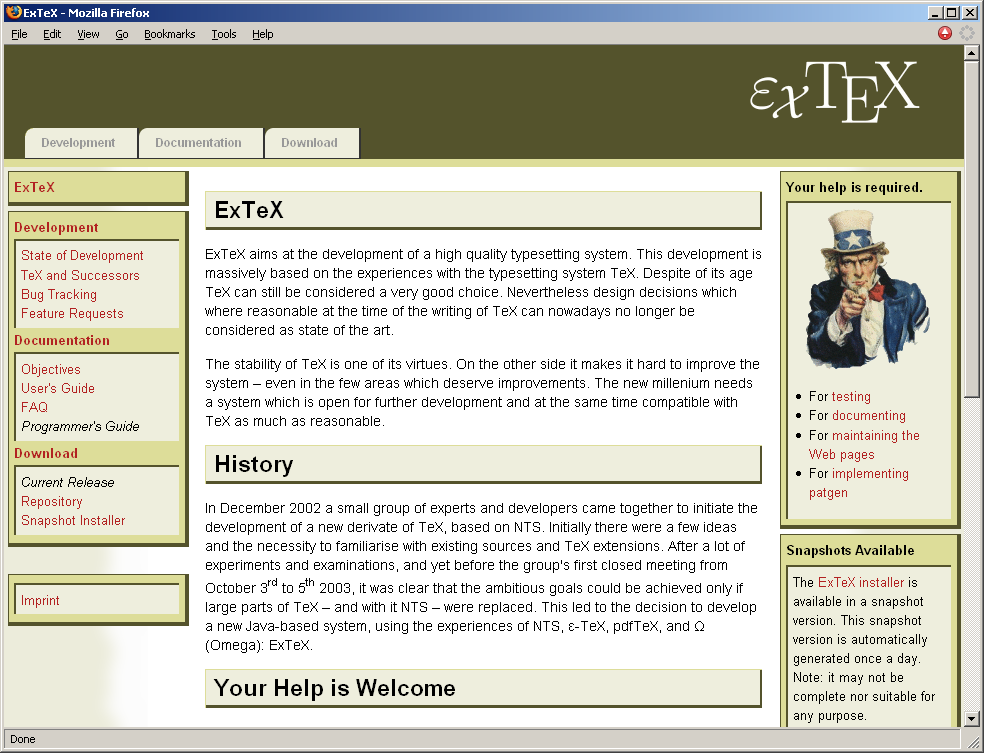
\includegraphics[scale=.4]{image/www-extex-org}
  \caption{www.extex.org}\label{fig:www-extex-org}
\end{figure}

The Web pages are build with a simple generator for a Web site written
in Perl. It has been made for \ExTeX. The aim is the ease of
maintainance for normal content of pages. They are stored as simple
HTML files and augmented automatically upon publication.

The layout is separated form the content and stored in several files.
This makes it very easy to adapt the appearance without touching the
contents.

The sources are kept in the subdirectory \texttt{src}. The generated
files are put into the subdirectory \texttt{www}. Both locations can
be configured.

To generate the Web site run the following command, where the current
directory is the directory \texttt{www}:

\begin{lstlisting}{}
#  make
\end{lstlisting}{}

This command creates a complete directory hierarchy with all necessary
sub-di\-rec\-to\-ries in \texttt{../target/www}. An exception are the
directories named \texttt{CVS}. Those directories are ignored.

The files starting with \verb|.| or ending in \verb|~| or in
\texttt{.bak} are also ignored. The files not ending in \verb|.html|
are copied into the destination tree. The files ending in \verb|.html|
are processed as follows: Text is inserted before the \verb|</head>|
tag from the file \File{.headEnd}. Text is inserted after the
\verb|<body>| tag from the file \File{.bodyStart}. Text is inserted
before the \verb|</body>| tag from the file \File{.bodyEnd}.

The text to be inserted is sought in the current directory and in case
of failure upwards in the super-directories until it is found. In the
inserted files the following entities and tags are replaced:

\begin{description}
\item [\tt\&top;]\ \\
  this is the relative path to the top directory.
\item [\tt\&year;]\ \\
  this is the current year when generating.
\item [\tt\&month;]\ \\
  this is the current month when generating.
\item [\tt\&day;]\ \\
  this is the current day when generating.
\item [\tt<tabs/>]\ \\
  this is replaced by the contents of the file .tabs.
\item [\tt<navigation/>]\ \\
  this is replaced by the contents of the file .navigation.
\item [\tt<info/>]\ \\
  this is replaced by the contents of the file .info.
\end{description}

Note, that even so it looks like XML processing, currently the
processing is based on string manipulation. Thus tricks possible with
XML might not work here.

\section{Layout}

The current layout has the scheme shown in figure~\ref{fig:www-layout}.
\definecolor{bg}{gray}{.95}
\begin{figure}[htbp]
  \centering

  \definecolor{bg}{gray}{.95}
  \definecolor{shadow}{gray}{.8}
  \begin{pgfpicture}{-1.25mm}{-5mm}{132mm}{51mm}
    
    \begin{pgftranslate}{\pgfpoint{22mm}{41mm}}
      \begin{pgftranslate}{\pgfpoint{1mm}{-1mm}}
        \color{shadow}
        \pgfmoveto{\pgfpoint{0mm}{0mm}} \pgflineto{\pgfpoint{5mm}{10mm}}
        \pgflineto{\pgfpoint{105mm}{10mm}} \pgflineto{\pgfpoint{100mm}{0mm}}
        \pgflineto{\pgfpoint{0mm}{0mm}} \pgffillstroke
      \end{pgftranslate}
      \color{bg}
      \pgfmoveto{\pgfpoint{0mm}{0mm}} \pgflineto{\pgfpoint{5mm}{10mm}}
      \pgflineto{\pgfpoint{105mm}{10mm}} \pgflineto{\pgfpoint{100mm}{0mm}}
      \pgflineto{\pgfpoint{0mm}{0mm}} \pgffillstroke
      \color{black}
      \pgfmoveto{\pgfpoint{0mm}{0mm}} \pgflineto{\pgfpoint{5mm}{10mm}}
      \pgflineto{\pgfpoint{105mm}{10mm}} \pgflineto{\pgfpoint{100mm}{0mm}}
      \pgflineto{\pgfpoint{0mm}{0mm}} \pgfstroke
      \pgfputat{\pgfpoint{52.5mm}{5mm}}{\pgfbox[center,center]{\sf\itshape Header}}
    \end{pgftranslate}
    
    \begin{pgftranslate}{\pgfpoint{18.5mm}{34mm}}
      \begin{pgftranslate}{\pgfpoint{1mm}{-1mm}}
        \color{shadow}
        \pgfmoveto{\pgfpoint{0mm}{0mm}} \pgflineto{\pgfpoint{2.5mm}{5mm}}
        \pgflineto{\pgfpoint{102.5mm}{5mm}} \pgflineto{\pgfpoint{100mm}{0mm}}
        \pgflineto{\pgfpoint{0mm}{0mm}} \pgffillstroke
      \end{pgftranslate}
      \color{bg}
      \pgfmoveto{\pgfpoint{0mm}{0mm}} \pgflineto{\pgfpoint{2.5mm}{5mm}}
      \pgflineto{\pgfpoint{102.5mm}{5mm}} \pgflineto{\pgfpoint{100mm}{0mm}}
      \pgflineto{\pgfpoint{0mm}{0mm}} \pgffillstroke
      \color{black}
      \pgfmoveto{\pgfpoint{0mm}{0mm}} \pgflineto{\pgfpoint{2.5mm}{5mm}}
      \pgflineto{\pgfpoint{102.5mm}{5mm}} \pgflineto{\pgfpoint{100mm}{0mm}}
      \pgflineto{\pgfpoint{0mm}{0mm}} \pgfstroke
      \pgfputat{\pgfpoint{52.5mm}{2.5mm}}{\pgfbox[center,center]{\sf\itshape Tab Bar}}
    \end{pgftranslate}
    
    \begin{pgftranslate}{\pgfpoint{-1mm}{2mm}}
      \begin{pgftranslate}{\pgfpoint{1mm}{-1mm}}
        \color{shadow}
        \pgfmoveto{\pgfpoint{0mm}{0mm}} \pgflineto{\pgfpoint{15mm}{30mm}}
        \pgflineto{\pgfpoint{35mm}{30mm}} \pgflineto{\pgfpoint{20mm}{0mm}}
        \pgflineto{\pgfpoint{0mm}{0mm}} \pgffillstroke
      \end{pgftranslate}
      \color{bg}
      \pgfmoveto{\pgfpoint{0mm}{0mm}} \pgflineto{\pgfpoint{15mm}{30mm}}
      \pgflineto{\pgfpoint{35mm}{30mm}} \pgflineto{\pgfpoint{20mm}{0mm}}
      \pgflineto{\pgfpoint{0mm}{0mm}} \pgffillstroke
      \color{black}
      \pgfmoveto{\pgfpoint{0mm}{0mm}} \pgflineto{\pgfpoint{15mm}{30mm}}
      \pgflineto{\pgfpoint{35mm}{30mm}} \pgflineto{\pgfpoint{20mm}{0mm}}
      \pgflineto{\pgfpoint{0mm}{0mm}} \pgfstroke
      \pgfputat{\pgfpoint{17.75mm}{15mm}}{\pgfbox[center,center]{\parbox{20mm}{\centering\sf\itshape
            Navigation\\Area~~~}}}
    \end{pgftranslate}
    
    \begin{pgftranslate}{\pgfpoint{22mm}{2mm}}
      \begin{pgftranslate}{\pgfpoint{1mm}{-1mm}}
        \color{shadow}
        \pgfmoveto{\pgfpoint{0mm}{0mm}} \pgflineto{\pgfpoint{15mm}{30mm}}
        \pgflineto{\pgfpoint{75mm}{30mm}} \pgflineto{\pgfpoint{60mm}{0mm}}
        \pgflineto{\pgfpoint{0mm}{0mm}} \pgffillstroke
      \end{pgftranslate}
      \color{bg}
      \pgfmoveto{\pgfpoint{0mm}{0mm}} \pgflineto{\pgfpoint{15mm}{30mm}}
      \pgflineto{\pgfpoint{75mm}{30mm}} \pgflineto{\pgfpoint{60mm}{0mm}}
      \pgflineto{\pgfpoint{0mm}{0mm}} \pgffillstroke
      \color{black}
      \pgfmoveto{\pgfpoint{0mm}{0mm}} \pgflineto{\pgfpoint{15mm}{30mm}}
      \pgflineto{\pgfpoint{75mm}{30mm}} \pgflineto{\pgfpoint{60mm}{0mm}}
      \pgflineto{\pgfpoint{0mm}{0mm}} \pgfstroke
      \pgfputat{\pgfpoint{37.5mm}{15mm}}{\pgfbox[center,center]{\sf\itshape
          Content Area}}
    \end{pgftranslate}
    
    \begin{pgftranslate}{\pgfpoint{85mm}{2mm}}
      \begin{pgftranslate}{\pgfpoint{1mm}{-1mm}}
        \color{shadow}
        \pgfmoveto{\pgfpoint{0mm}{0mm}} \pgflineto{\pgfpoint{15mm}{30mm}}
        \pgflineto{\pgfpoint{35mm}{30mm}} \pgflineto{\pgfpoint{20mm}{0mm}}
        \pgflineto{\pgfpoint{0mm}{0mm}} \pgffillstroke
      \end{pgftranslate}
      \color{bg}
      \pgfmoveto{\pgfpoint{0mm}{0mm}} \pgflineto{\pgfpoint{15mm}{30mm}}
      \pgflineto{\pgfpoint{35mm}{30mm}} \pgflineto{\pgfpoint{20mm}{0mm}}
      \pgflineto{\pgfpoint{0mm}{0mm}} \pgffillstroke
      \color{black}
      \pgfmoveto{\pgfpoint{0mm}{0mm}} \pgflineto{\pgfpoint{15mm}{30mm}}
      \pgflineto{\pgfpoint{35mm}{30mm}} \pgflineto{\pgfpoint{20mm}{0mm}}
      \pgflineto{\pgfpoint{0mm}{0mm}} \pgfstroke
      \pgfputat{\pgfpoint{17.5mm}{15mm}}{\pgfbox[center,center]{\parbox{20mm}{\centering\sf\itshape
            Info\\Area~~~}}}
    \end{pgftranslate}
    
    \begin{pgftranslate}{\pgfpoint{-1.25mm}{-5mm}}
      \begin{pgftranslate}{\pgfpoint{1mm}{-1mm}}
        \color{shadow}
        \pgfmoveto{\pgfpoint{0mm}{0mm}} \pgflineto{\pgfpoint{2.5mm}{5mm}}
        \pgflineto{\pgfpoint{102.5mm}{5mm}} \pgflineto{\pgfpoint{100mm}{0mm}}
        \pgflineto{\pgfpoint{0mm}{0mm}} \pgffillstroke
      \end{pgftranslate}
      \color{bg}
      \pgfmoveto{\pgfpoint{0mm}{0mm}} \pgflineto{\pgfpoint{2.5mm}{5mm}}
      \pgflineto{\pgfpoint{102.5mm}{5mm}} \pgflineto{\pgfpoint{100mm}{0mm}}
      \pgflineto{\pgfpoint{0mm}{0mm}} \pgffillstroke
      \color{black}
      \pgfmoveto{\pgfpoint{0mm}{0mm}} \pgflineto{\pgfpoint{2.5mm}{5mm}}
      \pgflineto{\pgfpoint{102.5mm}{5mm}} \pgflineto{\pgfpoint{100mm}{0mm}}
      \pgflineto{\pgfpoint{0mm}{0mm}} \pgfstroke
      \pgfputat{\pgfpoint{52.5mm}{2.5mm}}{\pgfbox[center,center]{\sf\itshape Footer}}
    \end{pgftranslate}
  \end{pgfpicture}

  \caption{Layout of the Web pages}\label{fig:www-layout}
\end{figure}

The Header contains the right aligned Logo only.
It is the same on all pages.
The Tab Bar shows the topmost navigation items with the Tab metophor.
The Navigation Area shows all navigation items.
It is the same on all pages.
The Info Area shows some info items specific for the current
navigation item.

The Content Area contains the contents of the page. This is maintained
by the site authors. The Footer contains a simple copyrigt note.


\section{Automatic Generation}

The web pages are generated automatically every night. This task is
performed with the help of a cron job on shell.berlios.de under the
account gene. In the course of this generation the current sources are
checked out from te CVS repository

Thus the normal user simply has to edit the pages in the area
\texttt{www/src} and check them into the CVS repository. The rest
happens automagically.

